% tikzpic.tex
\documentclass[crop,tikz]{standalone}% 'crop' is the default for v1.0, before it was 'preview'

\usetikzlibrary{arrows,decorations.pathmorphing,decorations.pathreplacing,backgrounds,positioning,fit,matrix}
\usetikzlibrary{shapes,calc,patterns,arrows.meta}
\tikzset{
	vert/.style={circle,inner sep=1.5,fill=white,draw,minimum size=.3cm},
	edge/.style={color=black, thick},
	diredge/.style={->,>={Stealth[width=8pt,length=8pt]},color=black, thick},
	timelabel/.style={fill=white,font=\footnotesize, text centered},
	wave/.style={decorate,decoration={coil,aspect=0}},
	dirwave/.style={->, >={Stealth[width=8pt,length=8pt]},decorate,decoration={coil,aspect=0}},
	diredge2/.style={->,>={Stealth[width=8pt,length=8pt]}}
}
\begin{document}
	
	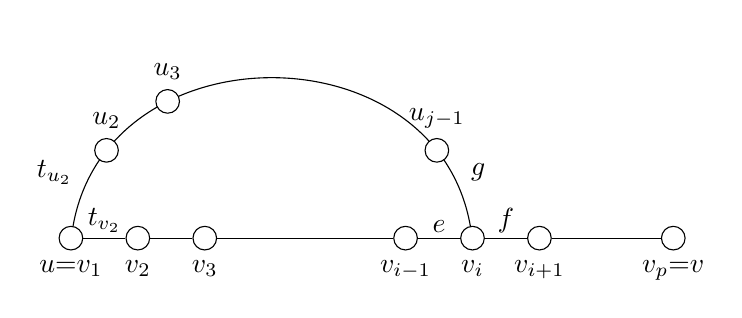
\begin{tikzpicture}[scale=.85]
		%%%S_uv
		\node[vert,label=below:$u{=} v_1$] (v1) at (1,0) {};
		\node[vert, label=below:$v_2$] (v2) at (2,0) {};
		\node[vert,label=below:$v_3$] (v3) at (3,0) {};
		\node[vert,label=below:$v_{i-1}$] (vi-1) at (6,0) {};
		\node[vert,label=below:$v_i$] (vi) at (7,0) {};
		\node[vert,label=below:$v_{i+1}$] (vi+1) at (8,0) {};
		\node[vert,label=below:$v_{p} {=} v$] (v) at (10,0) {};
		
		
		\draw (v1) -- node[label={above:$t_{v_2}$},yshift=-5] {} (v2) -- (v3) -- (vi-1) -- node[label={above:$e$},yshift=-5] {} (vi) -- node[label={above:$f$},yshift=-5] {} (vi+1) -- (v);
		
		\draw (v1) to [out=80,in=100,distance=3cm]
		node[pos=0.1,label={left:$t_{u_2}$}] {}
		node[vert,pos=0.15,label=above:$u_2$] {}
		node[vert,pos=0.3,label=above:$u_3$] {}
		node[vert,pos=0.85,label=above:$u_{j-1}$] {}
		node[pos=0.9,label={right:$g$}] {} (vi);
		
		%\draw[transform canvas={yshift=0mm}, blue]
		%(v1) -- (v2) -- (v3) -- node[pos=0.3,yshift=-2,label=above:$P_{u,v}$] {} (vi-1) -- (vi) ;
		
		%\draw[red]
		%(v1) edge[diredge2] [out=85,in=95,distance=2.1cm] node[pos=0.3,yshift=2,label=above:$P_{u,w}$] {} (v3) ;
	\end{tikzpicture}
	
\end{document}